\vspace{12pt}
\section{X-Ray Diffraction Analysis}

When a crystalline material is irradiated by monochromatic X-rays, diffraction patterns result due to constructive and destructive interference effects. Figure \ref{fig:XRD} illustrates the essential geometry of basic X-ray diffraction (XRD) measurements. In this research, bulk samples as well as thin films were subjected to XRD studies to analyze their crystalline structure. The angles at which constructive interference takes place can be used to determine the crystal structure of the material. Bragg’s Law, 
\begin{equation}
2 d \sin{\theta} = n \lambda,
\label{eq:bragg}
\end{equation}
relates the distance between the atomic planes $d$, and the diffraction angle 2$\theta$, where $\lambda$ is the wavelength of the X-ray radiation and $n$ is an integer. This relationship determines the type of planar configuration of the material, allowing for its identification and quantification.

\begin{figure}
\centering
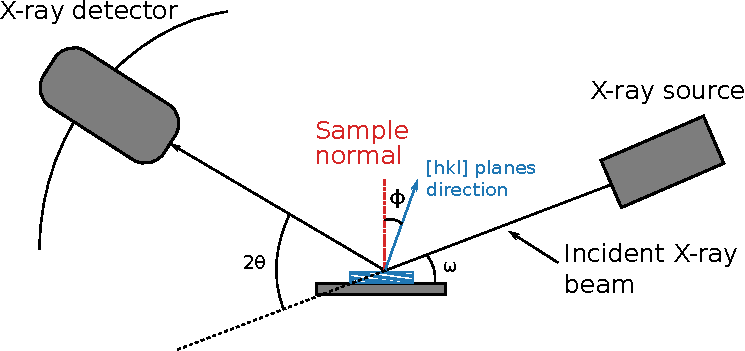
\includegraphics{Figures/XRD-2.pdf}
\caption[Schematic of X-ray diffraction.]{Schematic showing the geometry of X-ray diffraction. The diffraction angle 2$\theta$ and the incident angle $\omega$ are shown according to their standard definitions. The figure also depicts the situation in which the orientation of a particular family of lattice defines an ``offset'' angle $\phi$ with respect to the sample normal. In a single crystal, the indicated family of planes generates a scattering peak in an asymmetric scan. Other types of scan, as described in the text, permit systematic analysis of the crystal structure of a sample.}
\label{fig:XRD}
\end{figure}

This coherent scattering principle provides a powerful basis for analyzing the crystalline structure of bulk samples and thin film materials. The intensity of the diffracted X-ray photons varies with both, the diffraction angle 2$\theta$ and the incident angle $\omega$. A variety of different approaches have been developed in the field of crystallography for measuring the intensity of the diffracted X-rays depending on how 2$\theta$ and $\omega$ are varied during XRD angular scans \cite{Cullity2001}. Three methods are particularly relevant for this research. A first approach, known as the \emph{$2\theta$ scan}, is carried out by measuring the diffracted X-ray intensity as a function of 2$\theta$, for a fixed incident angle $\omega$. A second method, typically referred to as \emph{coupled scans}, measures the scattered X-ray intensity also as a function of 2$\theta$, but $\omega$ is made to change in a manner coupled to 2$\theta$, so that $\omega = (2\theta/2) + \phi$, where $\phi$ is the ``offset'' angle shown in Figure \ref{fig:XRD}. When $\phi=0$, a coupled scan is called a symmetric scan and is usually referred to as the \emph{$\theta$-2$\theta$ scan}. A coupled scan for which $\phi \neq 0$ is typically called an asymmetric, or \emph{$\omega$-2$\theta$ scan}. Finally, when diffracted intensities are also recorded as a function of the azimuthal angle of the sample (not shown in Figure \ref{fig:XRD}), the so-called \emph{pole figure measurements} can be carried out, in which quantitative assessments can be made of the fraction of grains in a polycrystalline material that exhibit preferential orientation. In the sections that follow, brief descriptions of these approaches are provided.

From an instrumentation point of view, two different instruments were used in this research for X-ray analysis. An X’pert thin film diffractometer (Philips, USA) with Cu K$\alpha$ radiation of wavelength $\lambda= 1.5418$ \AA\ was used for most of the XRD measurements in this project. The scan rate for all diffraction data obtained using this system was 0.01\textdegree/s for all samples. A more modern Empyrean diffractometer (Malvern Panalytical, USA), was also employed for some measurements. The same Cu K$\alpha$ radiation was used in this instrument, but which features a significantly stronger X-ray source, allowing faster measurements. The Empyrean unit also includes high resolution capabilities, which permits greater discrimination of angular position of reflections and studies of subtle changes in crystal unit cell sizes.   

\vspace{12pt}
\subsection{The $2\theta$ Scan}
The $2\theta$ scan, also often referred to as the ``Detector Scan,'' is particularly useful for polycrystalline materials where grains are randomly oriented. This type of  scan can be effectively used in phase identification studies because all reflections permitted for a given crystal symmetry and lattice are typically observed. In the case of thin films, the use of a small value of the incident angle $\omega$ (typically  $\omega \approx 2-3$\textdegree), causes the incident beam to have negligible penetration into the substrate, which essentially eliminates its diffraction signal. 

\vspace{12pt}
\subsection{Coupled Scans}
The lattice planes that are parallel to the surface facet of a single crystal bulk sample, or of an epitaxially-oriented thin film, are typically used to specify the orientation of the crystal under consideration. This set of planes, or any other family of planes in the single crystal, will satisfy the Bragg condition for constructive interference, only fortuitously in a $2\theta$ scan. For a chosen incident angle $\omega$, a crystal lattice may feature a family of planes with interplanar separation $d$ that causes equation \ref{eq:bragg} to hold for the  used $\lambda$ at a value of $2\theta$ within the range of the scan. If observed in the $2\theta$ scan, this reflection is only partly useful in characterizing the sample because it is very sensitive to $\omega$ and it does not capture the full picture of the crystal structure. Other epitaxial orientations that do not match the serendipitously fulfilled Bragg condition may be present in the sample and missed in the $2\theta$ scan. On the other hand, if a coupled $\theta$-2$\theta$ scan is performed, all families of planes that are oriented parallel to the surface will be detected within the range of the scan. For this reason, the $\theta$-2$\theta$ scan is the measurement of choice in samples suspected or known to be single crystals or exhibit epitaxial orientation. The tilting of the sample by a non-zero small offset angle $\phi$, causes the intensities of the single-crystal pattern of the coupled scan to rapidly decrease as the value  of $\phi$ is increased. This permits a straightforward confirmation of the single-crystal nature of the sample. Samples that were noted to be epitaxially-oriented thin films in this research were subjected to this XRD method of analysis.

\vspace{12pt}
\subsection{Pole Figure Measurements}
Crystallographic texture is one of the most important microstructural features underlying the properties of polycrystalline materials \cite{Kocks2000}. A well-established approach to measure texture in a polycrystalline material is to collect the sum of lattice plane reflections from a large number of crystallites, as a function of the polar ($\alpha$) and azimuthal ($\beta$)  angles of the sample with respect to the laboratory frame of reference. This is routinely carried out using a four-circle goniometer \cite{Kocks2000} by varying the polar angle typically from 0\textdegree{} to 85\textdegree{} and the azimuthal angle from 0\textdegree{} to 360\textdegree{} with step increments of 5\textdegree. The diffracted intensity of the X-ray beam at each ($\alpha$, $\beta$) coordinate can be displayed as a contour plot in a so called ``pole figure,'' which effectively exhibits the density of crystallite axes (or poles), for any given family of crystal lattice planes, oriented along the direction normal to the surface.   
The pole figure contour plots are usually constructed using equal-area projection and the pole densities can be normalized by that of a hypothetical sample with random orientation and expressed in units of multiples of random distribution.

In this research, measurements of crystallographic texture were performed on select thin film samples by XRD in reflection geometry using a 3-axes goniometer. X-ray pole figures were collected for select reflections of BaZrO$_3$ by varying the polar angle with the standard parameters mentioned above ($\alpha$ = 0\textdegree{} to 85\textdegree{}; $\beta$ = 0\textdegree{} to 360\textdegree{}) with a step increment of 5\textdegree{} and a scan time of 4 s per step. The pole figures were not corrected for background and defocusing of the incident beam, and therefore represent a qualitative assessment of general texturing trend in the analyzed thin films.